\section{Assumptions}
\label{sec:assumptions}
\autoref{fig:events} shows how complex even the initial events during a
collision are. As it would be too difficult to analyse these subsequent
situations without the proper software, only the first event (A) is
taken into account to reduce the complexity. To decrease the complexity even
more, a number of assumptions are made. In the following paragraphs these
assumptions are explained in detail.

Our victim is a healthy thirty year old male with a height of 1,80m and a mass
of 80kg. Using \autoref{fig:proportions}, we estimate the distance from
respectively the angle, knee and hip to the ground to be 0,07m, 0,51m and 0,95m.
The lower legs has a mass of 3,72kg and the upper legs has a mass of
8kg\cite{Ob}. The car weighs 2400kg,  the bull bar is made of 
aluminium ($E_{Al}$=69 GPa and $\nu_{Al}$=0,32)
%stainless steel ($E_{SS}$=210 GPa and $\nu_{SS}$=0,305
%\footnote{\url{http://www.engineeringtoolbox.com/poissons-ratio-d_1224.html}})
and its most protuding part sits at 0,80m heigh. \cite{huiskes1977geometrical}
suggest $E_{femur}$ = 20 GPa and $\nu_{femur}$ = 0,37.

\begin{figure}[htp]
\begin{center}
  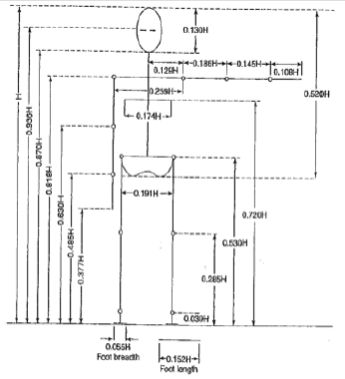
\includegraphics{img/proportions.png}
  \caption{Various lengths of human body segments in proportion to
  total height.}
  \label{fig:proportions}
\end{center}
\end{figure}

Before the collision the pedestrian is located right in front of the car.
He is walking and at the moment of the crash the leg closest to the car is in
stand phase. The other leg is in swing phase. We examine the femur of the former
leg, because it is most likely to fail. The weight of both his upper and lower
leg segments are also calculated. It is assumed the weight is equally
distributed over the length of both parts, so the center of gravity is situated
in the middle of both parts.

At the time of collision the car is decelerating, but it still has a speed of 36
km/h (10 m/s). Due to the bullbar that is mounted on the bumper, the initial
contact between the body of the pedestrian and the car is limited to
the bar touching the upper leg of the pedestrian. The femur is the long
bone that provides support in the upper leg. Around the femur the hamstring
muscles, the quadriceps muscles and a layer of fat act as shock absorbers
during the impact. The literature suggests using a damping factor of roughly
15\% \cite{kannus1999comparison}.

As only the initial phase of the impact is considered in this paper, it is
assumed that the horizontal velocity of the hip is zero at the time of impact.
% TODO herschrijven
The foot also remains in place, but rotates inwards at the ankle. Because of
this the bones in the lower leg do not deform. Further it is assumed that the
knee does not bend initially. So the deformation induced by the bull bar is only
reflected in the femur shaft. In reality the knee will also be affected by the
forces exerted by the bull bar. Depending on the situation and the relative strength of
both, the femur will break or the knee will be distorted. In the following
analysis however, it is assumed that the femur will absorb the initial impact.
This means we assume that the knee will not become distorted (so it will
continue to properly connect the upper and lower leg) and that the other bones
-- from pelvis to the little bones in the foot -- are not affected initially.
Because of these (rather rough) assumptions the whole leg can be treated as one
structure which is clamped at the top (pelvis) and with a hinge at the level of
the ankle. The force exerted on this structure by the bull bar is treated as a
force concentrated in one point at a height of 80 cm. It is assumed that the
bull bar will not deform during the collision, nor that the crumple zone of the
car is activated.

In \autoref{fig:hyper1} the complex system of the leg of the pedestrian getting
hit by the bull bar of the car is visualised. In order to make a mechanical
analysis of this system a number of assumptions had to be made. To make the
assumptions three things were taken into consideration. First,
\cite{snedeker2005assessing} proposed a set of boundary conditions to analyse
the impact of a car bumper on the leg of a pedestrian. In this paper it is
suggested to assume the pelvis to be �fixed� -- such that the pelvis has a
horizontal velocity of zero -- during the first moments of the crash. Second, we
analysed the deformation of a set of mechanical systems and compared these with
our visual analysis of the legs of dummies in crash
tests\footnote{\url{https://www.youtube.com/watch?v=tNRHB75NiIc}}. The main
parts in all mechanical systems were the pelvis (suggestions: clamped, simply
supported or hinge), the femur (suggestion:
a beam), the knee (suggestions: hinge, simple supported or simply a
uninterrupted beam which represents femur, knee and bones in lower leg), the
bones in the lower leg (a beam) and the foot and ankle (suggestions: clamped,
simply supported or hinge). For all combination of the mechanical
representations of these main mechanical parts the line of deformation was
drawn. Finally, the system represented in \autoref{fig:hyper1} was chosen.

 \begin{figure}[htp]
\begin{center}
  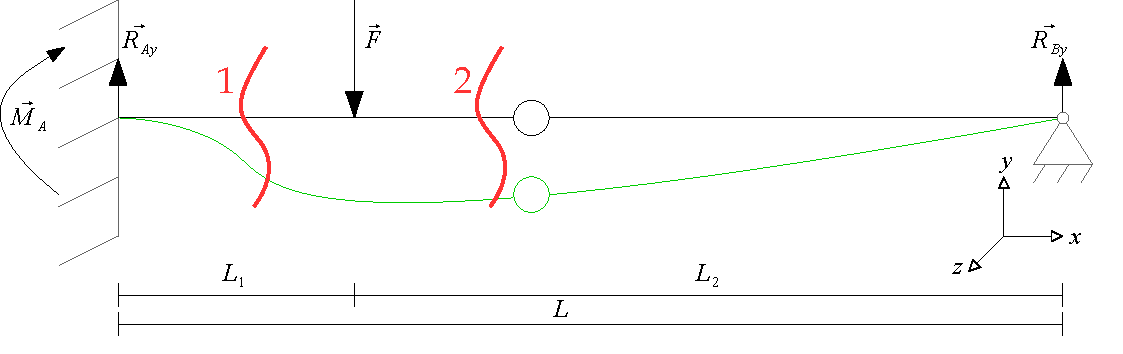
\includegraphics[page=1,width=\textwidth]{img/hyper.pdf}
  \caption{Schematic of the system under consideration. The pelvis (left) is
  modeled as a clamp, while the angle (right) is replaced by a hinge. The knee
  (circle) is merely added for visual guidance, it does not play any
  significant part in this analysis. The total length $L$ is split up in $L_1$
  and $L_2$ at the point of impact.}
  \label{fig:hyper1}
\end{center}
\end{figure}

As the pedestrian is a young male it is assumed he has normal bones, not
affected by any disease. The femoral bone has an average length of 48 cm, a
shaft diameter of 2.43 cm and the femoral canal has a diameter of 13
mm.\footnote{http://www.orthopaedicsone.com}
